\documentclass[aspectratio=169,UTF8,11pt]{ctexbeamer}

\usetheme{Madrid}
\usecolortheme{default}
\setbeamertemplate{navigation symbols}{}
\setbeamertemplate{footline}[frame number]

\usepackage{amsmath,amssymb,amsthm,mathtools}
\usepackage{booktabs}
\usepackage{hyperref}

% 图形与颜色
\usepackage{graphicx}
\usepackage{xcolor}
\usepackage{tikz}

% TikZ 常用库（讲 TikZ 时通常很有用）
\usetikzlibrary{arrows.meta,calc,positioning,decorations.pathreplacing}

% 表格与排版
\usepackage{booktabs}
\usepackage{array}
\usepackage{multirow}

% 超链接
\usepackage{hyperref}

% 标题信息
\title{TikZ 使用简介}
\author{Crazyfish}
\institute{ZJU Math}

\begin{document}

\begin{frame}
  \titlepage
\end{frame}


\begin{frame}{什么是 TikZ？为什么使用它？}

\textbf{TikZ} 是 LaTeX 中常用的绘图工具，
可以直接在文档源码中绘制几何图形、函数示意图、流程图与结构图。

\textbf{TikZ 的主要特点：}
\begin{itemize}
  \item 与 LaTeX 文档无缝结合，字体、公式风格统一；
  \item 图形由代码生成，便于修改、复现与版本管理；
  \item 可以直接在图中插入数学公式与符号；
  \item 适合绘制的内容：坐标系与函数图像、几何示意图、箭头关系图与流程图、简单网络图与结构图
  \item TikZ 不是“插入图片”，而是“\alert{用 LaTeX 代码描述图形}”。
\end{itemize}
\end{frame}


\begin{frame}[fragile]{TikZ 的几种常见使用方式}
\small

\begin{enumerate}
    \item \textbf{嵌入在普通文档中：} 适合论文、讲义、作业中的局部示意图
\begin{verbatim}
\begin{tikzpicture}
  \draw (0,0) -- (2,1);
\end{tikzpicture}
\end{verbatim}
    \item \textbf{行内小图：} 使用 \verb|\tikz| 命令，适合在正文中插入简单符号或小示意
\begin{verbatim}
这是正文中的一个小图：\tikz \fill (0,0) circle (2pt);
\end{verbatim}
    \item \textbf{独立文档方式：} 适合将一幅图单独编译成 PDF，再插回主文档
\begin{verbatim}
\documentclass[tikz,border=3pt]{standalone}
\usepackage{tikz}
\begin{document}
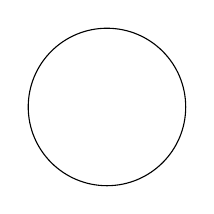
\begin{tikzpicture}
  \draw (0,0) circle (1cm);
\end{tikzpicture}
\end{document}
\end{verbatim}
\end{enumerate}
\end{frame}

\begin{frame}[fragile]{基本图形命令：线、矩形、圆、箭头}
\small

\textbf{常见绘图命令：}

\begin{itemize}
  \item \textbf{线段与折线}（坐标单位默认是 cm）
\begin{verbatim}
\draw (0,0) -- (1,1) -- (2,0);
\end{verbatim}

  \item \textbf{矩形}
\begin{verbatim}
\draw (0,0) rectangle (2,1);
\end{verbatim}

  \item \textbf{圆}
\begin{verbatim}
\draw (0,0) circle (1cm);
\end{verbatim}

  \item \textbf{箭头}
\begin{verbatim}
\draw[->] (0,0) -- (2,0);
\end{verbatim}

  \item \textbf{样式选项}
\begin{verbatim}
\draw[thick, dashed, red] (0,0) -- (2,1);
\end{verbatim}
常见样式包括：
  \verb|thick|, \verb|dashed|, \verb|red|, \verb|blue|, \verb|->|, \verb|<-|, \verb|<->|。
\end{itemize}
\end{frame}

\begin{frame}[fragile]{节点 \texttt{node}：给图形加文字标注}
\small

\textbf{常见用法：}

\begin{itemize}
  \item \textbf{在线上加标注}
\begin{verbatim}
\draw (0,0) -- (2,0) node[midway, above] {$a$};
\end{verbatim}

  \item \textbf{单独放置节点}
\begin{verbatim}
\node at (1,1) {$A$};
\end{verbatim}

  \item \textbf{带边框的节点}
\begin{verbatim}
\node[draw] at (0,0) {Start};
\end{verbatim}

\item \textbf{常见位置参数（相对标记的点）：}\verb|above|：上方，\verb|below|：下方，\verb|left|：左侧，
\verb|right|：右侧

\item \textbf{常见位置参数（相对标记的路径）：}\verb|midway|：路径中点，\verb|near start|：靠近起点，
\verb|near end|：靠近终点
\end{itemize}
\end{frame}


\begin{frame}[fragile]{坐标与相对位置：让作图更自然}
\small

\begin{itemize}
    \item \textbf{绝对坐标：} 用 $(x,y)$ 直接指定位置
\begin{verbatim}
(0,0), (1,2)
\end{verbatim}
    \item \textbf{相对坐标：} 基于已有点或已有路径通过矢量运算得到新位置.
\begin{verbatim}
\draw (0,0) -- ++(1,1) -- ++(1,-1);
\end{verbatim}
    \item \textbf{网格辅助：}
\begin{verbatim}
\draw[step=1cm, gray!30] (0,0) grid (3,2);
\end{verbatim}
\end{itemize}
\end{frame}

\begin{frame}[fragile]{\texttt{scope} 与局部样式}
\small

\textbf{基本思想：}
当一组图形共享同样的颜色、线宽或其他样式时，
可以用 \texttt{scope} 将它们放在一起，统一设置局部样式。

\textbf{示例：}
\begin{verbatim}
\begin{tikzpicture}
  \draw (0,0) -- (1,0);
  \begin{scope}[blue, thick]
    \draw (0,1) -- (1,1);
    \draw (0,2) -- (1,2);
  \end{scope}
  \draw (0,3) -- (1,3);
\end{tikzpicture}
\end{verbatim}

\textbf{说明：}
\begin{itemize}
  \item \texttt{scope} 内的图形自动继承 \verb|blue, thick|；
  \item \texttt{scope} 外的图形不受影响；
  \item 适合管理复杂图形中的局部设置。
\end{itemize}
\end{frame}

\begin{frame}[fragile]{曲线与 Bézier 曲线}
\small

\textbf{基本思想：}
除了直线以外，TikZ 还可以绘制曲线。
常见方式是使用 Bézier 曲线，通过控制点决定弯曲形状。

\vspace{0.6em}

\textbf{示例：}
\begin{verbatim}
\begin{tikzpicture}
  \draw (0,0) .. controls (1,1) and (2,1) .. (3,0);
\end{tikzpicture}
\end{verbatim}

\vspace{0.6em}

\begin{itemize}
  \item 曲线从 \verb|(0,0)| 出发，到 \verb|(3,0)| 结束；
  \item 两个控制点 \verb|(1,1)| 和 \verb|(2,1)| 决定曲线如何弯曲；
  \item 控制点并不一定在曲线上，但会影响曲线形状。
\end{itemize}

\vspace{0.4em}

\begin{block}{应用}
Bézier 曲线常用于弯曲箭头、光滑连接线以及几何示意图中的弧形路径。
\end{block}

\end{frame}


\begin{frame}[fragile]{\texttt{foreach} 循环}
\small

\textbf{基本思想：}
当图中有许多重复元素时，可以使用 \texttt{foreach} 自动生成，
避免一条一条重复书写。

\vspace{0.6em}

\textbf{示例：重复画圆}
\begin{verbatim}

\begin{tikzpicture}
  \foreach \x in {0,1,2,3}
    \draw (\x,0) circle (0.2);
\end{tikzpicture}
\end{verbatim}

\textbf{说明：}
\begin{itemize}
  \item \verb|\x| 是循环变量；
  \item 每次循环都会把当前数值代入代码中；
  \item 非常适合生成刻度、网格点、节点列等重复结构。
\end{itemize}

\vspace{0.4em}

\begin{block}{作用}
\texttt{foreach} 可以显著缩短代码，并提高绘图效率与可维护性。
\end{block}

\end{frame}

\begin{frame}[fragile]{\texttt{pgfplots}：高质量函数图与数据图}
\small

\texttt{pgfplots} 是建立在 TikZ/PGF 之上的绘图库，
专门用于绘制函数图像、实验数据图和统计图。
\begin{itemize}
  \item 自动生成坐标轴、刻度、网格和图例；
  \item 可直接绘制数学函数，如 $y=x^2$、$\sin x$；
  \item 可读取表格数据并绘制曲线、散点图、柱状图；
  \item 与 LaTeX 数学公式和字体风格自然统一。
  \item 适用场景：数学函数图像，数值实验结果图，收敛曲线、误差曲线，对数坐标图、散点图、柱状图等
\end{itemize}

\textbf{基本用法：}
\begin{verbatim}
\usepackage{pgfplots}  % 依赖包
\pgfplotsset{compat=1.18} % 版本兼容
\begin{tikzpicture}
  \begin{axis}[xlabel=$x$, ylabel=$y$]
    \addplot[domain=0:2] {x^2};
  \end{axis}
\end{tikzpicture}
\end{verbatim}
\end{frame}
\end{document}
